\chapter{配置开发环境}
本实验指导书\footnote{本章节部分参考网络博文 \url{https://panqiincs.me/2019/07/26/develop-stm32-on-linux/}.}将使用 Arch Linux 作为开发环境操作系统, 以 STM32CubeMX\footnote{意法半导体公司推出的跨平台工程创建与管理软件.} 创建新工程 (当然我们也会为每一个 lab 提供设置好的空白工程用以学习), 使用 GNU 工具链\footnote{\url{https://developer.arm.com/tools-and-software/open-source-software/developer-tools/gnu-toolchain/gnu-rm}.}进行 ARM 嵌入式开发的编译和调试, 以及使用 VS Code 进行代码编辑. 以上提及的软件都是跨平台的, 读者可以在 Windows 操作系统下尝试, 但需要注意配置 PATH 路径等问题.

\section{安装 GNU 工具链}
假设读者处于普通未提权账户环境, 打开终端, 键入如下的指令并回车, 以安装对应平台的编译器, 调试器与函数库:

\begin{minted}{bash}
sudo pacman -Syu arm-none-eabi-{gcc,gdb,newlib}
\end{minted}

这里添加了 \texttt{-yu} 的命令选项, 以强制更新仓库数据库和操作系统. 这是 Arch Linux 官方建议的行为.

\section{安装 STM32CubeMX}
若读者安装了 AUR helper (例如 yay\footnote{\url{https://github.com/Jguer/yay}.}), 可以直接在普通账户终端执行

\begin{minted}{bash}
yay -S stm32cubemx
\end{minted}

然后不断回车进行下一步即可. 若没有安装, 可以在一个空间较大的临时目录下进入终端, 执行如下的命令:

\begin{minted}{bash}
git clone https://aur.archlinux.org/stm32cubemx.git
cd stm32cubemx
makepkg -si
\end{minted}

效果与使用 AUR helper 类似.

若不想使用 AUR 提供的 STM32CubeMX, 可以在意法半导体官网\footnote{\url{https://www.st.com/en/development-tools/stm32cubemx.html}.}下载最新版本. 这是一个图形化界面的安装器. 可以注册 ST 账户后登录下载, 也可以以访客身份下载 (需要填写简单的个人信息, 然后在接收到的邮件中得到认证方可进行下载).

下载完成后解压, 应当能看到类似这样命名的文件: \texttt{SetupSTM32CubeMX-<版本号>}, 同时还有一个名为 \texttt{jre} 的文件夹. 在终端中定位到该文件所在目录, 保证 \texttt{jre} 文件夹相对位置不变的情况下, 在终端中执行:

\begin{minted}{bash}
chmod +x SetupSTM32CubeMX-<版本号>
./SetupSTM32CubeMX-<版本号>
\end{minted}

然后在打开的安装器内不断点 Next 继续安装即可.

\section{安装 VS Code 与编辑器环境}
安装过程类似使用 AUR helper 安装 STM32CubeMX:

\begin{minted}{bash}
yay -S visual-studio-code-bin
\end{minted}

然后就可以在开始菜单中找到 VS Code 的快捷方式.

随后需要提前配置编辑器环境. 进入 VS Code, 在左侧一栏找到 Extensions 按钮或使用 Ctrl+Shift+X 快捷键, 在展开的扩展程序页面搜索 ``clangd'' 插件\footnote{\url{https://clangd.llvm.org/}.}并启用, 如图 \ref{fig:1-env clangd} 所示:

\begin{figure}[H]
    \centering
    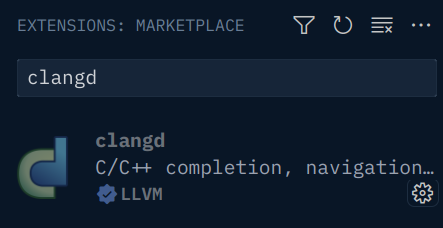
\includegraphics{images/1-env-clangd.png}
    \caption{扩展程序页面 ``clangd'' 搜索结果}
    \label{fig:1-env clangd}
\end{figure}

clangd 插件适用于 CMakeLists 编译环境, 但我们将要以更加简单的 Makefile 作为我们的编译环境, 因此需要安装额外的软件用以生成 clangd 插件的配置:

\begin{minted}{bash}
sudo pacman -Syu bear
\end{minted}

对于该软件的使用, 将放在后续章节讲解.

\section{安装 stm32flash 与配置串口}
Linux 上没有 Windows 上那些简单好用的图形化烧录工具. 这里我们选择的是开源的命令行工具 stm32flash\footnote{\url{https://sourceforge.net/projects/stm32flash/}.}. 它同样可以在 AUR helper 中安装:

\begin{minted}{bash}
yay -S stm32flash
\end{minted}

随后我们需要安装 CH340 芯片驱动, 这样才可以使用专用线在电脑和开发板之间串口通讯. 首先我们需要检查系统中是否存在该驱动. 在终端中执行如下命令:

\begin{minted}{bash}
lsmod | grep ch34
\end{minted}

如果有诸如 ``ch341'', ``ch34x'' 的输出, 则表示安装了该驱动, 无需如下的操作. 若结果为空白, 则在终端中执行如下命令:

\begin{minted}{bash}
git clone https://github.com/juliagoda/CH341SER
cd CH341SER
make
sudo make load
\end{minted}

此时再键入 \texttt{lsmod | grep ch34}, 应当有如下类似的输出:

\begin{minted}{text}
ch34x                  36864  0
\end{minted}

配置好驱动之后, 就需要检查开发板串口信息. F4 系列霸天虎开发板上 BOOT0 引脚应该默认用跳线帽与 GND 接地引脚连接, BOOT1 (PB2) 引脚默认与 GND 接地引脚连接. 根据 STM32 的相关文档, 此时开发板启动时将进入主闪存存储器启动模式, 加载内置 Flash 存储的用户程序. 但是使用 stm32flash 烧录用户程序, 必须使开发板进入系统存储器的启动模式加载 bootloader. STM32 的三种启动模式如下表 \ref{tab:1-env boot} 所示:

\begin{table}[H]
    \centering
    \caption{STM32 的三种启动模式} \label{tab:1-env boot}
    \begin{tabular}{ccc} \toprule
        \textbf{BOOT0} & \textbf{BOOT1} & \textbf{启动模式}      \\\midrule
        GND (低电平)      & 任意             & 主闪存存储器 (用户程序)      \\
        3V3 (高电平)      & GND (低电平)      & 系统存储器 (bootloader) \\
        3V3 (高电平)      & 3V3 (高电平)      & 内置 SRAM            \\
        \bottomrule
    \end{tabular}
\end{table}

具体方法是, 拔除 BOOT0 和 GND 连接的跳线帽, 用跳线帽或杜邦线连接 BOOT0 和 3V3 引脚, 再按动开发板上的复位按钮或上电, 即可让开发板进入 bootloader. 此时我们就可以使用专用线进行串口通讯了. 终端执行 \texttt{ls /dev} 后应该能找到一个类似于 \texttt{ttyUSB0} 的设备文件. 使用 stm32flash 检查串口的信息的命令如下:

\begin{minted}{bash}
sudo stm32flash /dev/ttyUSB0
\end{minted}

若成功引导开发板进入 bootloader, 应当有类似于如下的输出:

\begin{minted}{text}
stm32flash 0.7

http://stm32flash.sourceforge.net/

Interface serial_posix: 57600 8E1
Version      : 0x31
Option 1     : 0x00
Option 2     : 0x00
Device ID    : 0x0413 (STM32F40xxx/41xxx)
- RAM        : Up to 128KiB  (12288b reserved by bootloader)
- Flash      : Up to 1024KiB (size first sector: 1x16384)
- Option RAM : 16b
- System RAM : 30KiB
\end{minted}

另外, 若没有成功引导 (例如仍然以主闪存存储器启动), 则会输出 \texttt{Failed to init device} 类似的错误.

在之后的实验调试时, 烧录用户程序后记得将 BOOT0 引脚重新连接 GND 引脚并复位. 为方便起见, 可以准备一个面包板.
